%From: Lisa C Jeffrey <jeffrey@math.ias.edu>
%Date: Thu, 8 May 1997 21:33:50 -0400

\documentclass[12pt]{article}
\usepackage[dvips]{epsfig}
\begin{document}

\newcommand{\printname}[1]
        {\smash{\makebox[0pt]{\hspace{-1.0in}\raisebox{8pt}{\tiny #1}}}}
%\newcommand{\labell}[1] {\label{#1}\printname{#1}}
\newcommand{\labell}[1] {\label{#1}}
\input amssym.def
\input amssym.tex




\def\h{\frak h}
\def\tr{{\rm tr}}
\def\Ad{{\rm Ad}}
\def\u{\bf  u}
\def\O{{\cal O}}
\def\calo{{\cal O}}
\def \calh{{ \cal H} }
\def \cald{{ \cal D} }
\def \call{{ \cal L} }
\def\tA{\tilde A}
%\def\qdet{\text{qdet}}
\def\k{\kappa}
\def\RR{\Bbb R}

\def\ad{{\rm ad}}
\def\Hom{{\rm Hom}}

\def\g{\frak g}
\def\lieg{\frak g}


\def\ZZ{\Bbb Z}
\def\CC{\Bbb C}
\def\d{\partial}


\def\Tr{{\rm Tr}}


\def\<{\langle}
\def\>{\rangle}


%\def\RE{\text{Re}}

\def\Id{{\rm Id}}
\def\End{{\rm End}}
\def \gauge{{\cal G}}
\def \liegauge{{\bf  g}} 
\def \lieh {{\bf h}}
\def \fn { {\rm{ Fun}} }
\def \voll{ {\rm Vol} }
\newcommand{\eqdef}{\stackrel{{\rm def} }{=} }
\newcommand{\areaa}{ {\bf a} }

%\topmatter

\begin{center}
{\large \bf Lecture II-10: Quantum gauge theories in two dimensions and
intersection theory on moduli spaces}
\end{center}

\centerline {\bf Edward Witten} 
%\endtopmatter

\centerline{Notes by Lisa Jeffrey}

{\bf 10.1. The partition function in two dimensional Yang-Mills theory.}

We consider gauge theories in two dimensions with a simple gauge
group $G$. The spacetime is a compact
Riemann surface $\Sigma$ of genus
$g$ with no boundary.
To apply our methods 
to intersection  theory on moduli spaces, we shall need to consider
the case $G = SU(n)/\ZZ_n$ and consider bundles on $\Sigma$ for which
the transition functions do not lift to $SU(n)$: in mathematical
terms we are considering the
moduli space of holomorphic vector bundles on $\Sigma$  with rank 
$n$ and degree $d$.

The theory we consider is {\it{physical Yang-Mills theory}.}
The fields are a $G$ connection $A$ on a 
$G$ bundle $P$ on $\Sigma$, with 
curvature $F_A$; 
the Lagrangian is 
\begin{equation} \labell{10.1}
{\cal L}=\frac{1}{4e^2}\int d^2x\left(|*F_A|^2\right).
\end{equation}

The partition function is thus
\begin{equation} \labell{10.2}
 Z = \frac{1}{ {\rm Vol}  (G)} \int D A e^{ - {\cal L} }.
\end{equation}
We introduce a scalar field $\phi$ with values in $\ad(P)$ 
and rewrite the path integral for the partition function as 
\begin{equation} \labell{10.3}
 Z = \frac{1}{\voll (G)} \int DA D \phi \exp \{
i \int \Tr \phi F - \frac{e^2}{2} \int d\mu \Tr \phi^2 
\}. 
\end{equation}
This theory is invariant under area preserving diffeomorphisms since it
has no explicit dependence on a Riemannian metric on $\Sigma $ but
only on the {\it{measure}}
   $d\mu = * (1)$. 
It is clear that the theory depends only on
the coupling constant $e$ and  
   the area $\areaa$ of $\Sigma$ only 
through the combination  $e^2 \areaa$.
The path integral  (\ref{10.3}) is well behaved
under taking  the limit as 
$e \to 0$.

We make a further modification to the path integral for the partition 
function by introducing a fermionic variable $\psi$ which is a one-form
in the adjoint representation (in other words $\psi$ is an element of
of $\Omega^1(\Sigma)  \otimes \Gamma(\ad P)$. The field $\psi$ should
be thought of as lying in the tangent space to the space $\cal A$ of 
connections on $\Sigma$. 
The path integral becomes
\begin{equation} \labell{10.4}
Z = \frac{1}{\voll G} \int DA D\phi D \psi \exp \{ i \int_\Sigma 
\Tr (\phi F) + \frac{1}{2} \int \Tr (\psi \wedge \psi) 
- \frac{e^2}{2} \int d\mu \Tr (\phi^2) \}.  
\end{equation}
Since the Lagrangian in (\ref{10.4}) contains no terms which involve both 
$\psi $ and the other fields $\phi$ and $A$, we can integrate out
$\psi$ and recover the earlier expression (\ref{10.3}).

We can now define a supersymmetry operation 
$\delta$ on the space of fields:
\begin{equation} \labell{10.5}
 \delta A = i \psi, 
\end{equation}
\begin{equation} \labell{10.6}
 \delta \psi = - d_A \phi 
\end{equation}
\begin{equation} \labell{10.7}
 \delta \phi = 0 
\end{equation}
It follows that 
$\delta^2 A = - i d_A \phi, $ in other words $\delta^2 = 0 $ up to the
action of a gauge transformation.
(Here, $d_A$ refers to the de Rham differential $d$ twisted by a 
connection $A$ on $\Sigma$.) 
We may check the invariance of the action under $\delta$: we have
\begin{equation} \labell{10.8}
 \delta \int \Tr (\phi F) = - i  \int \Tr (\phi D_A \psi), 
\end{equation}
while 
\begin{equation} \labell{10.9}
 \delta \int \Tr (\psi \wedge \psi) = - \int \Tr (D_A \phi  \wedge \psi).
\end{equation}
After integrating by parts, we find that the action appearing in 
(\ref{10.4}) is invariant.


{\bf 10.2. A finite dimensional analogue: the Cartan model.}

Our path integral is a path integral over the infinite dimensional
space $\cal A$ of connections which is acted on by the 
gauge group $\gauge$ with Lie algebra ${\rm Lie}(\gauge)$.
The {\it{Cartan model}} is 
used to treat a  finite dimensional analogue of this situation:
for a more detailed description see Chapter 7 of {\bf [BGV]}.
The analogue of $\cal A$ is a finite dimensional manifold $M$
equipped with the action of a compact Lie group $H$ (which is the 
analogue of $\gauge$). Functions of $A$ and $\psi$ correspond to 
differential forms on $M$, while the analogue of 
functions of $A, \psi$ and $\phi$ are elements of 
$\Omega^*(M) \otimes \fn (\lieh)$. In fact we restrict to the 
$H$-invariant subspace 
$\Bigl ( \Omega^* (M) \otimes \fn (\lieh) \Bigr )^H $ where
$H $ acts in the obvious way on $\Omega^*(M)$ and acts on 
$\lieh$ (and hence on $\fn (\lieh))$ via the adjoint action.
Here $\fn (\lieh)$ denotes an appropriate class of functions 
on $\lieh$: in the literature one most usually restricts to 
polynomial functions ${\rm Pol} (\lieh) = S(\lieh^*)$ (the symmetric algebra
on $\lieh^*$). 

The set 
$$\Omega^*_H(M) = 
\Bigl ( \Omega^* (M) \otimes S(\lieh^*) \Bigr )^H $$ has a 
natural grading: it is the differential form grading plus two times the
polynomial grading (in other words a linear function on $\lieh$ is 
assigned grading $2$). With this grading one sees that both terms in the
operator\footnote{Mathematicians normally  use a convention in which
the $i$ in (\ref{difdef}) is omitted.}
\begin{equation} \labell{difdef}
 D = d  - i \iota_{V(\phi)} 
\end{equation}
increase the grading by 1. (Here $d$ is the de Rham differential and
$\iota_{V(\phi)} $ is the interior product with the vector field
$V(\phi)$ induced on $M$ by the action of $\phi \in \lieh$.)
We may write
$$ \iota_{V(\phi)} = \sum_a \phi^a \iota_{V^a}, $$
introducing a basis $\{\phi^a\}$ for $\lieh$. It is easy to check
(since we have restricted to $H$-invariant elements of 
$\Omega^*(M) \otimes S(\lieh^*))$ that
$D^2 = 0 $, so one may take the cohomology with respect to $D$: this cohomology
is identified with the $H$-equivariant cohomology $H^*_H(M)$ 
of $M$.\footnote{Throughout this lecture 
all cohomology groups will be
assumed to have complex coefficients.}
If $H$ acts freely on $M$ the topological 
quotient $M/H$ is a manifold (and $M$ is a principal $H$-bundle over
$M/H$), and the equivariant cohomology is identified with the ordinary 
cohomology $H^*(M/H)$ of the quotient. 

We shall start with classes in the $D$-cohomology  of $\Omega^*_H(M)$.
One type of classes come from $(S(\lieh)^*)^H$ (in other words, 
the  polynomials on the Lie algebra $\lieh$ which
are invariant under the adjoint action): this
is identified with the $H$-equivariant cohomology of a point,
or in other words with the cohomology $H^*(BH)$ of the 
classifying space $BH$. 
If 
$M$ is a principal $H$-bundle over $M/H$ 
(or equivalently if the action of $H$ on $M$ is 
free) then each  invariant
polynomial on 
$\lieh$ corresponds to a characteristic class 
of   principal bundles with structure group $H$. Under the 
isomorphism $H^*_H(M) \cong H^*(M/H)$, the invariant
polynomial $S$ on $\lieh$ is identified with the corresponding
characteristic class of the principal $H$-bundle  $M$. (This
is given in  Chern-Weil theory as  $S(F_A)$  where $A$ is a 
connection on the bundle $M \to M/H$ and $F_A$ is its curvature,
which is a 2-form on $M$ with values in $\lieh$).

\def\cala{ {\cal A} }
\def\opso{ {\cal O}_S^{(0)} }
\def\opsone{ {\cal O}_S^{(1)} }
\def\opstwo{ {\cal O}_S^{(2)} }
\def\moduli{ {\cal M} }

{\bf 10.3 Infinite dimensional Cartan: the descent equations}

We shall now outline the analogue of the Cartan model in our 
infinite dimensional situation: this material 
is covered in Section 3.3 of {\bf [W2]}.
  The space $M$ is the infinite dimensional
vector space  $\cala$ of connections on a $G$ bundle $P$ over a 
Riemann surface $\Sigma$. We start with an $\Ad$-invariant 
polynomial $S$ on the Lie algebra $\lieg$; from this
we shall construct  an operator
$ \opso$ in two dimensional Yang-Mills theory, which 
corresponds to a cohomology class in the moduli space $\moduli$.
Recall that the field theory contained a field $\phi$ with 
values in $\lieg$. 
We define 
\begin{equation} \labell{10.10}
 \opso = S(\phi).
\end{equation}
The object $\opso$ is thus a function on $\Sigma$:
we shall see that up to the supersymmetry differential 
$\delta$, the operator $\opso(p) = S(\phi(p))$ is independent of 
the choice of a point $p$ $\in \Sigma$.
We decompose the field $\phi$ into 
components $\{\phi^b\}$ (where $b$ indexes
a basis for $\lieg$). 
Then
\begin{equation} \labell{10.11}
 d \opso = \sum_b \frac{\partial S}{\partial \phi^b} d_A \phi^a 
\end{equation}
\begin{equation} \labell{10.12}
 = i \delta (\sum_b \frac{\partial S}{\partial \phi^a} \psi^b ),
\end{equation}
in terms of the supersymmetry operator $\delta$.
Thus if we define
$$\opsone = -  \sum_b \frac{\partial S}{\partial \phi^b} \psi^b , $$
we have 
proved
\begin{equation} \labell{10.13}
d \opso = - i \delta \opsone. 
\end{equation}
Here $\opsone$ should be viewed as  a 1-form on $\Sigma$.

We can iterate this procedure: we find that
\begin{equation} \labell{10.14}
 d \opsone = \sum_{a,b} \frac{\partial^2 S}{\partial \phi^a \partial \phi^b}
D_A \psi^a \wedge \psi^b  + \sum_a \frac{\partial S}{\partial \phi^a} 
D_A \psi^a.
\end{equation}

Observing that $D_A \psi = \delta F_A$, we can convert (\ref{10.14}) into
$ d \opsone = - i \delta \opstwo$, where
we have defined
\begin{equation} \labell{10.15}
\opstwo = \frac{1}{2} \sum_{a,b} 
 \frac{\partial^2 S}{\partial \phi^a \partial \phi^b}
 \psi^a \wedge \psi^b  + i  \sum_a \frac{\partial S}{\partial \phi^a} F_a.
\end{equation}
\newcommand{\que}[2]{Q_{#1}^{(#2)} }
These equations may be summarized as follows:
\begin{equation} \labell{10.16}
 (d + i \delta) (\opso + \opsone + \opstwo) = 0. \end{equation}
(The point is that in an appropriate double complex
the total differential is $d + i\delta$ and 
$\opso + \opsone + \opstwo $ is closed.)

We shall now use this to construct cohomology classes on the 
moduli space 
\begin{equation} \labell{10.17}
\moduli = \cala^{\rm flat}/\gauge. 
\end{equation}
 If we choose a $q$-cycle $C$ in 
$\Sigma$, we find (using Stokes' theorem) that
$$ \que{S}{q}(C)  \eqdef \int_C \calo_S^{(q)} $$ 
satisfies
\begin{equation} \labell{10.18}
 \delta \que{S}{q}(C) = 0, 
\end{equation}
and
if $C = \delta B$ is a boundary, then 
\begin{equation} \labell{10.19}
 \que{S}{q}(C) = \delta T ~\mbox{for some }~T. 
\end{equation} 
Provided that the group $\gauge$ of gauge transformations acts
freely on $\cala$,  the $\que{S}{q}(C)$ correspond to the 
generators of the cohomology of $\moduli$:
they are 
cohomology classes on ${\cal A}/\gauge$ which  we will restrict 
to the moduli space $\cala_{\rm flat}/\gauge$. 
 These generators are 
given in Section 2 of {\bf[AB]}: they are produced by
taking the slant product of the characteristic
classes of the {\it universal bundle} over $\moduli \times \Sigma$ 
with classes in the homology of $\Sigma$. 
The quantum field theory will compute a generating functional
\begin{equation} \labell{10.20}
 \int_{\moduli} \exp \Bigl \{ \alpha \que{S}{0}(p)  + 
\sum_{j = 1}^{2g} \beta_j \que{S'_j}{1}(C_j) + \gamma \que{S''}{2}(\Sigma) 
\Bigr \}
\end{equation}
which will encode all  intersection numbers in the cohomology 
of $\moduli$. A mathematical proof of these formulas for intersection 
numbers is given in {\bf [T]} for the case $G = SU(2)$ and in 
{\bf [JK2]} in the case $G = SU(n)$ (in those
cases where the moduli space $\moduli$ is smooth).
Here, $p$ is a point in $\Sigma$, 
 the $C_j$ are $2g$ cycles in 
$\Sigma$ corresponding to the homology $H_1(\Sigma)$,
and the $S$, $S'_j$ and $S''$ are arbitrary
invariant polynomials on $\lieg$ (which are in general distinct).
For simplicity we shall mostly treat the case $G = SU(2)$, for which
the ring of invariant polynomials on $\lieg$ is a polynomial ring
on one generator $S$ given by 
$$ S(\phi) = \Tr(\phi^2). $$



\def \cali{{\cal I}}

{\bf 10.4 Equivariant integration and localization}

We now return to the finite-dimensional situation of 
Section 10.2. 
We would like to define a map
$ {\cali}: Z^*_H(M) \to \CC$
(where $ Z^*_H(M)$ are the $D$-closed elements in $\Omega^*_H(M)$)
by integrating over $M \times \lieh$. In order to define a
convergent integral, we introduce a convergence
factor $e^{- \varepsilon \Tr (\phi^2) } $.
(In fact in the  mathematical treatment of this 
convergence factor one may replace the 
Gaussian $e^{- \varepsilon \Tr (\phi^2) } $ by any collection 
of rapidly decreasing functions $\{f_\varepsilon\}$ on $\lieh$ 
which (as $\varepsilon \to 0$) represent the Dirac delta distribution:
see {\bf [JK1]} for a mathematical treatment of  equivariant 
integration in the Cartan model.)
For $\alpha  \in Z^*_H(M)$ we define
\begin{equation} \labell{10.21}
 \cali (\alpha) = 
\int_{\phi \in \lieh} \int_{M}
 d \phi_1 \dots d \phi_s 
e^{- \varepsilon \Tr (\phi^2) }  \alpha (\phi) . 
\end{equation}



\def\eqw{\tilde{\omega}}

In fact in order to ensure convergence of  the integral (\ref{10.21})  we must
place some hypotheses on  $\alpha$.
A useful class of equivariantly closed forms are obtained in the special
case when $M$ is a symplectic manifold with symplectic form $\omega$,
and the action of $H$ on $M$ is Hamiltonian with moment map 
$\mu: M \to \lieh^*$:
We see readily that 
\begin{equation} \labell{eq:eqsym}
\eqw = -i \Tr (\phi \mu) + \omega 
\end{equation}
satisfies
$$ D \eqw = 0$$ 
(where $D$ is the Cartan model differential defined by 
(\ref{difdef})).

The computation of the integral (\ref{10.21}) will be governed by 
a localization principle similar to that which leads to the 
Duistermaat-Heckman formula for an oscillatory integral over a 
symplectic manifold with a Hamiltonian torus action. 
We choose an $H$-invariant 1-form $\lambda$ for which
\begin{equation} \labell{10.22}
D \lambda = d \lambda + - i (V(\phi), \lambda);
\end{equation}
where $V(\phi)$ is the vector field given by the action of 
$\phi$ (which of course depends linearly on $\phi$). The integral (\ref{10.21})
is not changed by replacing
$\exp ( - \varepsilon \Tr (\phi^2)  )  $ by 
$\exp (  - \varepsilon \Tr (\phi^2)  +   i t D \lambda ) $ 
since $\exp (it D \lambda)$ expands as  $1 + it D \lambda + \dots$ 
Because $-t D \lambda = i t (V (\phi), \lambda) - t (d \lambda)$, 
as $t \to \infty$ the integral localizes around points where
$(V (\phi), \lambda) = 0 $. We may see this by alternatively 
computing the partition function by completing the
square and performing the integral
over $\phi$: to leading order in $t$ this gives a factor
$$ \exp - \frac{t^2}{4\varepsilon} \sum_a |(V_a, \lambda)|^2, $$
so by considering the
behaviour for $\epsilon \to 0$ 
we see that the integral localizes around points where
$(V_a, \lambda) = 0 $ for all $a$. 

We now specialize to the case where $M$ is a symplectic
manifold equipped with the Hamiltonian action of a compact
group $H$: the moment map will be denoted 
$\mu$. We define $I = |\mu|^2: M \to \RR$, 
the norm squared of the moment map. We may choose an almost
complex structure $J \in {\rm End} (TM)$  compatible with the symplectic
structure, and let $\lambda = J (dI) $ be the invariant 
one-form defined above. The points where $(V_a, \lambda) = 0 $ 
are readily identified with the critical points of $I$.
We see this because
$$ d I = 2 \sum_a \mu_a d\mu_a, $$
so since $V_a = \omega^{-1} d\mu_a $
(regarding the symplectic form $\omega$ as an isomorphism 
$T_x M \to T_x^* M$ for each $x \in M$, with 
inverse $\omega^{-1}: T_x^* M \to T_x M$) we have
$$ \omega^{-1} dI = 2 \sum_a \mu_a V_a. $$
Here $dI \in \Omega^1(M) $, so 
$\omega^{-1} dI$ should be regarded
as an element of $\Gamma (TM).$ 
Thus $(V_a, \lambda) = 0 $ implies 
$(\omega^{-1} dI , \lambda) = 0 $,
in other words
$$ (\omega^{-1} dI, J (dI) ) = 0 $$
(where both sides of this equation are in $\Gamma(TM)$).
This implies $dI = 0 $ since $\omega$ and $J$ combine
to give a nondegenerate symmetric bilinear form $g$ on the
cotangent space,
defined by 
$$g(X,Y) = \omega^{-1}(X, JY) $$
(for $X, Y \in \Gamma (T^* M)$). 
Thus our integral formally localizes on the critical
points of $I$. One obvious source  of such critical points 
is $\mu^{-1} (0)$, but there are other critical points where
$I \ne 0 $. 

We now give a derivation of (one version of) the Duistermaat-Heckman
formula.
As noted above,
the form (\ref{eq:eqsym}) 
$\eqw = -i \Tr (\phi \mu) + \omega $ is equivariantly closed. 
We may thus compute
\begin{equation} \labell{eq:dh}
\frac{1}{\voll H} \int_{\phi\in \lieh} 
d\phi_1 \dots d\phi_n \int_M 
\exp  \Bigl ( -i \Tr (\phi \mu) + \omega \Bigr ) . 
\end{equation}
(Note that if we did not include the integration  over $\phi$
in the formula (\ref{eq:dh}), the oscillatory integral 
over $M$ would correspond to a sum over the components of the
fixed point set of $T$: see for instance Chapter 7 of {\bf [BGV]}.)
If however we first integrate over $\phi$ we obtain a delta function
$\delta (\mu) $, so the formula becomes
$$
 \frac{1}{\voll H} 
\int_M 
\exp  \omega \delta (\mu) = \int_{\mu^{-1} (0)/H} e^\omega $$
in other words the symplectic 
(Liouville) volume of the symplectic quotient $\mu^{-1} (0)/H$.


We wish, however, also to include a factor 
$\exp ( - \varepsilon \Tr (\phi^2) )$ in the integrand. 
Thus we wish to compute 
\begin{equation} \labell{eq:nonabdh}
Z (\varepsilon) \eqdef \frac{1}{\voll H} \int_{\phi\in \lieh} 
d\phi_1 \dots d\phi_n \int_M 
 \alpha \exp  \Bigl ( -i \Tr (\phi \mu) + \omega - \varepsilon 
\Tr (\phi^2) \Bigr ) ,
\end{equation}
where $\alpha = \alpha(\phi) $ is an equivariantly closed form  on $M$ which 
has \emph{polynomial} dependence on $\phi$. 
We assume $H$ acts freely on $\mu^{-1}(0)$; 
near $\mu^{-1}(0)$, the equivariantly closed class
$\Tr (\phi^2) $ (which comes from the $H$-equivariant cohomology of a 
point in the Cartan model) is the pullback of a 
class $\Theta $ on the symplectic quotient $\mu^{-1}(0)/H$, which
is the class which would be evaluated in Chern-Weil theory as 
$\Tr (F_B^2)$  if $B$ is a connection on the principal $H$-bundle
$\mu^{-1}(0) \to \mu^{-1}(0)/H$ and $F_B$ is its curvature. 
Similarly, near $\mu^{-1}(0)$, $\alpha$ restricts to the pullback
of a class $\hat{\alpha} $ on $\mu^{-1}(0)/H$.

We find  that 
$$ Z(\varepsilon) = \int_{\mu^{-1}(0)/H} 
\hat{\alpha} \exp (\omega - \varepsilon \Theta) 
+ O (e^{-b/\varepsilon}), $$
where $b$ is the smallest nonzero critical value of $I$. 
To see heuristically why the nonzero critical value $b$ of
$I$ should give a contribution to the integral 
(\ref{eq:nonabdh}) which is of order $e^{-b/\varepsilon}$, 
we compute (\ref{eq:nonabdh}) by first integrating out $\phi$ 
(assuming for simplicity that $\alpha = 1$). We compute the
integral over $\phi$ by completing the square in $\phi$, 
which gives 
$$ Z (\varepsilon) = \int_{M} \exp  \left (\omega - \frac{1}{\varepsilon}
\Tr (\mu^2) \right ). $$








{\bf 10.5 Equivariant integration: the infinite dimensional case}

We now pass to the 
infinite dimensional case and 
study  the path integrals corresponding to 
equivariant integration. Recall that we had defined
the generating functional (\ref{10.20}).
We restrict to 
$G = SU(2)$ or $SO(3)$; we will pick the 
invariant polynomials $S, S'_j$ and
$S''$ to  all be   equal to the generating
polynomial  (denoted $S$), namely
$S(\phi)  = {\rm Tr} (\phi^2)$. 
(We have picked an ${\rm Ad}$-invariant inner product on 
$\lieg$, which is denoted $\Tr$; 
 a corresponding measure is defined on $G$.)
We assume $\gamma = 1$  and $\alpha = - e^2/2$ in 
(\ref{10.20}), and observe that 
for $S = \Tr (\phi^2)$ we have 
$$\que{S}{1}(C_j)  = \int_{C_j} \Tr (\phi \psi). $$ 
Thus the path integral that gives rise to (\ref{10.20}) 
becomes (where $p$ is a point in $\Sigma$)
\begin{equation} \labell{eq:dhgauge}
Z(e,\{ \beta_j\}) =  \frac{1}{\voll G} \int \cald A \cald \psi \cald \phi 
e^{ \{ - \frac{e^2}{2}  \Tr (\phi^2) (p)  + 
\sum_{j = 1}^{2g} \beta_j \int_{C_j} \Tr (\phi \psi) +
\int_{\Sigma}  \que{S}{2} 
 \} }.
\end{equation}
(Note that when $S (\phi) = {\rm Tr} (\phi^2), $ the
object $\int_{\Sigma}  \que{S}{2} $ corresponds to the 
symplectic form on $\cala$, and  becomes identified with
 the standard symplectic form on the moduli space 
$\cal M$.)

We can now see how the  integral 
(\ref{eq:dhgauge}) can be rewritten in such a way that
the generating functional (\ref{10.20}) involving
the $\que{S}{q}$  for $q = 0,1,2$ is equated with a corresponding
generating functional involving only $\que{S}{q}$ for $q = 0,2$.
This is accomplished by performing the integral over $\psi$, which
is Gaussian: completing the square to 
perform this integral we see that
we pick up a term 
\begin{equation} \labell{eq:dhgauge2}
 \frac{1}{\voll G}  \int \cald A \cald \phi
\exp \Bigl \{ i \int_\Sigma \Tr (\phi F_A) - \varepsilon \Tr (\phi^2) (p) , 
\Bigr \}
\end{equation}
where $\varepsilon = e^2/2 - \sum_{i < j} 
\beta_i \beta_j \# (C_i \cap C_j). $
In other words we can eliminate the odd-dimensional 
generators of the cohomology ring of the moduli space
corresponding to $\que{S}{1}$ (the non-algebraic cycles in the 
moduli space).
A mathematical version of this argument is given 
in the work of Thaddeus {\bf [T]}.



{\bf 10.6 The partition function of Yang-Mills theory}

The following material is covered in 
Section 4 of {\bf [W2]}.
We have now reduced the formula we need to compute to the
partition function  (\ref{10.2})
of  Yang-Mills theory  without the fermionic variable $\psi$ included. 
To compute the partition function we quantize the theory. 
 This is
accomplished by replacing the Riemann surface by a cylinder $C \times [0,T]$
of length $T$  (where $C \cong S^1$ should be  regarded as space and 
is assumed to have length $L$, while 
$[0,T]$ is a time interval of length $T$). 
The space of fields is equal to the space of connections 
$\cala_C$ on the circle $C$, so the Hilbert space is 
$$ \calh = C^\infty (\cala_C)^\gauge,$$
 the 
gauge invariant functions on $\cala_C$. Since up to gauge
equivalence all connections are classified by their holonomy
around the curve $C$, we find that 
the Hilbert space is identified with 
$$
\calh = C^\infty (G)^G, $$
the ring of  functions on $G$ which are invariant under the
adjoint action (or equivalently the functions on the maximal 
torus $T$ which are invariant under the action of the Weyl group).
The Hilbert space is thus identified with the irreducible 
(complex) representations
$R$ of $G$ (or equivalently with their characters which
are denoted $\chi_R$ or $\Tr_R$): we take
the characters $\chi_R$ to form a basis of $\calh$, or 
$$ \calh = \oplus_R \CC_{(R)} .$$
For every irreducible representation $R$ the basis element
$\chi_R $ is identified with a function 
$\Psi_R$ on $\cala_C$, namely
$$ \Psi_R(A) = \chi_R ({\rm Hol}_C A ). $$

The Hamiltonian of the theory is 
$$ H = -\frac{e^2}{2} \int_C \Tr |F_{01}|^2 $$ 
(where $F_{01}$ is the curvature of the connection), which becomes
(identifying the Hamiltonian as an operator on $\calh$ in terms of the
position variables $A^b (\theta)d\theta $ on $\cala_C$ and the corresponding
momentum variables $(\partial A^b(\theta)/\partial t) d\theta$
 which are identified
with $ - i  \partial /\partial A^b (\theta) $ under canonical 
quantization) 
$$ H = \frac{e^2}{2} \int_C \Tr ( \frac{\delta}{\delta A})^2. $$
The action of the operator $ \delta/\delta A^a(\theta) $ on $\Psi_R$ gives 
$$ \frac{\delta}{\delta A^a(\theta)}  \Tr_R {\rm Hol}_C (A) = 
\Tr_R T^a {\rm Hol}_C (A) $$
in terms of a basis  $T^a$ for the Lie algebra $\lieg$ of $G$. 
We thus see that 
\begin{equation} \labell{eq:quadcas}
\sum_{a} \frac{\delta}{\delta A^a(\theta)} 
\frac{\delta}{\delta A^a(\theta)}
\Tr_R {\rm Hol}_C (A) = 
\Tr_R ( \sum_a T^a T^a  {\rm Hol}_C (A)). 
\end{equation}
The element $\sum_a T^a T^a$ is the  {\it quadratic Casimir}
of $G$, whose evaluation in the representation $R$ is 
denoted 
$$ \Tr_R \sum_a T^a T^a \eqdef c_2(R). $$
Thus we see that 
\begin{equation} \labell{eq:hamact}
H \Psi_R = \frac{e^2 c_2(R) L}{2} \Psi_R. 
\end{equation} 
We thus see that
\begin{equation} \labell{eq:hameval}
< \Psi_R| e^{ -H T} | \Psi_R> = 
\exp ( - e^2 c_2(R) LT/2 ) = \exp (- e^2\areaa c_2 (R)/2 ), 
\end{equation}
in terms of the area $\areaa = LT$ of the cylinder. 
The answer depends only on the combination $e^2 \areaa$. 

\newcommand{\eulconst}{\alpha}

In fact the effect of renormalization in this quantum field theory
is to introduce a factor of the form
\begin{equation} \labell{undet}
\exp ( \eulconst \int_\Sigma d \mu {\cal R} 
 + (e^2/2) \beta \int_\Sigma d \mu )
\end{equation}
into the integrand (where
$\cal R $ is the Riemann curvature
and  $\eulconst$ and $\beta$ are appropriately chosen 
real-valued constants).
 The effect of the term 
involving $\beta$ is to change the quadratic 
Casimir $c_R$ to a renormalized value
$\tilde{c}_R$ which
differs from $c_R$ by addition 
of a constant. The factor $\eulconst$ multiplies the
Euler characteristic of $\Sigma$: it will eventually
be adjusted to ensure that the overall
normalization of the partition function and
its dependence on the genus $g$ agrees with that found by other
methods (for instance by computing the partition function 
when $\varepsilon = 0 $ using Reidemeister-Ray-Singer
torsion, as in Section 4 of {\bf [QYM]}).
 %%%%%

\newcommand{\pants}{ {\cal P} }
\newcommand{\operp}{ {  \hat{ \que{S}{0}}(p)  } }

\begin{figure}
\centerline{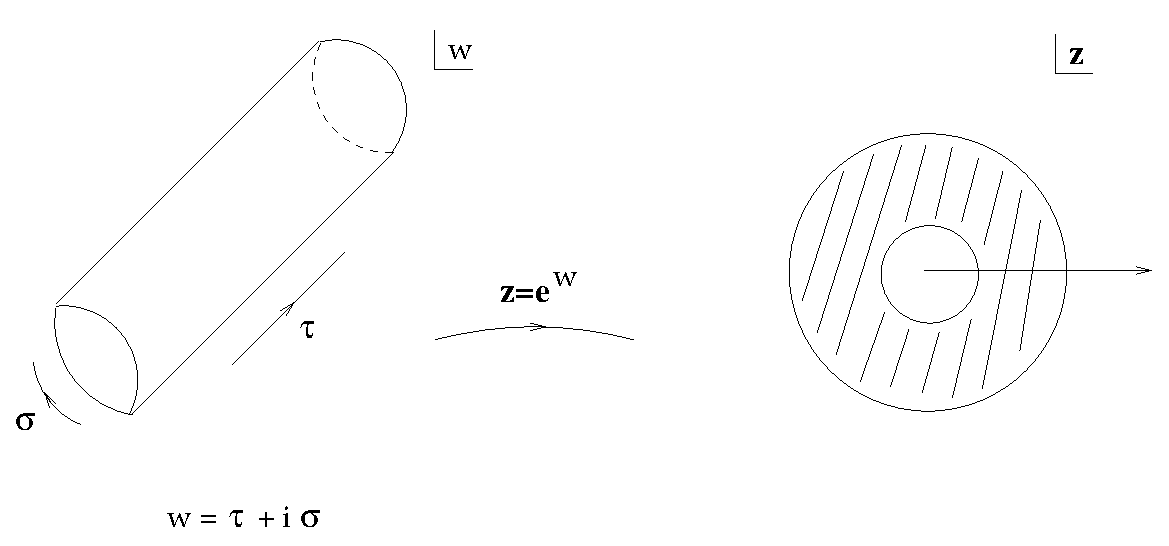
\epsfig{file=fig1.eps}}
\end{figure}

\begin{figure}
\centerline{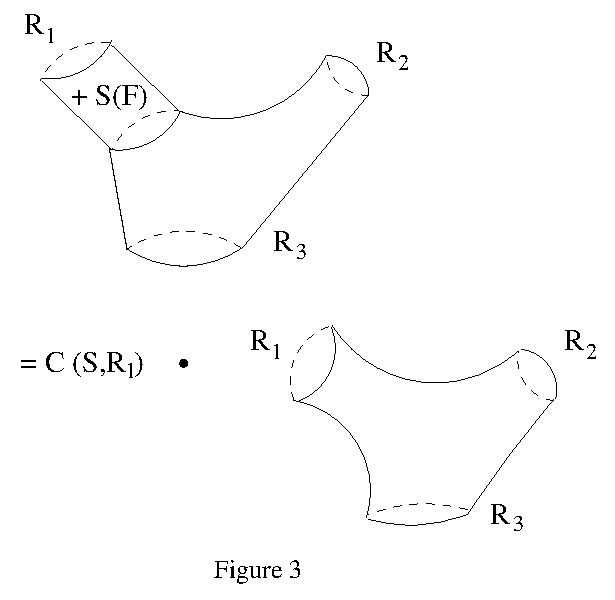
\epsfig{file=fig3.eps}}
\end{figure}

We must also consider the field theory on the Riemann surface 
${\cal P}$ which
is a sphere with three disks removed (the trinion or pair of pants:
see Figure~1).
If we insert the operator 
$\hat{ \que{S}{0} } (p)   $ corresponding to the
observable $\que{S}{0}(p) $ (where $p$ is some point in 
$\cal P$) we see using (\ref{eq:hamact}) and its
generalizations that the state 
$\Psi_R$ is an eigenstate of $\operp$ with some eigenvalue 
$C(S,R)$:
\begin{equation} \labell{eigval}
\operp \Psi_R = C(S,R) \Psi_R. 
\end{equation}
Here, if $S$ is an invariant polynomial of degree $l$ on 
$\lieg$, $C(S,R)$ is the corresponding $l$-th order Casimir of the
representation $R$. By considering the one point function 
determined by the Riemann surface ${\cal P}$ with the operator
$\operp$ inserted near the $j$-th
boundary component (see Figure 3), we find that this one
point function is equal to 
$C(S, R_j) W_{R_1 R_2 R_3}$ (for $j = 1, 2, 3$) if 
$W_{R_1 R_2 R_3}$ is the partition function for $\cal P$ with 
states $\Psi_{R_1}, $ $\Psi_{R_2}, $  $\Psi_{R_3} $  along the
three boundary components. This does not depend on the 
 boundary component $j$ (since this
field theory is invariant under area
preserving diffeomorphisms): it follows that the 
Casimirs $C(S, R_j)$ are all equal, and since this is true for all
invariant polynomials $S$, we must have
$R_1 = R_2 = R_3$ if $W(R_1, R_2, R_3) \ne 0$. 

We are thus reduced to computing the partition function of $\cal P$ with
boundary conditions determined by the external 
state $\Psi_R$ along all three boundary components. Denote the value
of this partition function in the limit of zero area 
by $w_R$: more generally for a pair of pants $\cal P$ of area $\areaa $
one
obtains
\begin{equation} \label{partpants}
Z_R = w_R \exp ( - \tilde{c}_2 (R) \frac{\areaa e^2}{2} ). 
\end{equation}
  
     We now consider the problem of computing the partition function
for a Riemann surface of genus $g$ with no boundary. Such a surface may
be formed by gluing together $2g-2$ copies ${\cal P}_j$ 
of $\cal P$ along
$3g-3$ boundary circles $C_\gamma$. We may factor the path integral for
the partition function according to the values of the fields restricted
to the boundary circles $C_\gamma$. If 
$A'  $ denotes the value of a connection 
on the boundary circles $\coprod_\gamma C_\gamma $ of the 
${\cal P}_j$, and 
$\cala_{A'} = \{ A \in \cala: 
A|_{\coprod_\gamma C_\gamma}  = A' \}$  is the set of 
all connections which restrict to a  given boundary
value $A'$, we have
\begin{equation}
\int \cald A e^{- \call} = 
\int \cald A' \int_{\cala_{A'}} e^{- \call}
\end{equation}
(cf. {\bf [QYM]}, Section 4.5).
Once we have fixed the boundary values $A'$, the space
$\cala_{A'}$ is the product of 
$2g-2$ copies of the space of connections on $\pants$ (with prescribed
boundary values). In quantization the partition function of 
$\pants$ is 
\begin{equation} 
Z(\pants, A|_{\partial \pants}) = \sum_R w_R \prod_{\gamma = 1}^3 
\Psi_R (A|_{C_\gamma} ). 
\end{equation}
To recover the partition function for the closed 
Riemann surface $\Sigma$ of genus $g$, we multiply 
$2g-2$ copies of $Z(\pants)$ and integrate over the
boundary values $A'$.
Using the orthogonality relations for the group characters
which correspond to the states
$\Psi_R$, we find
\begin{equation}
Z (\Sigma) = 
\sum_R w_R^{2g-2} \exp (  - \frac{e^2 \areaa \tilde{c}_2 (R)} {2}  ). 
\end{equation}

We now explain how to compute the $w_R$. We observe that the 
partition function for a disk $D$ of area $\areaa$ with an external
state $\Psi_R $ on the boundary is 
\begin{equation} 
Z(D) = v_R  \exp (  - \frac{e^2 \areaa \tilde{c}_2(R)} {2}  ).
\end{equation}

\begin{figure}
\centerline{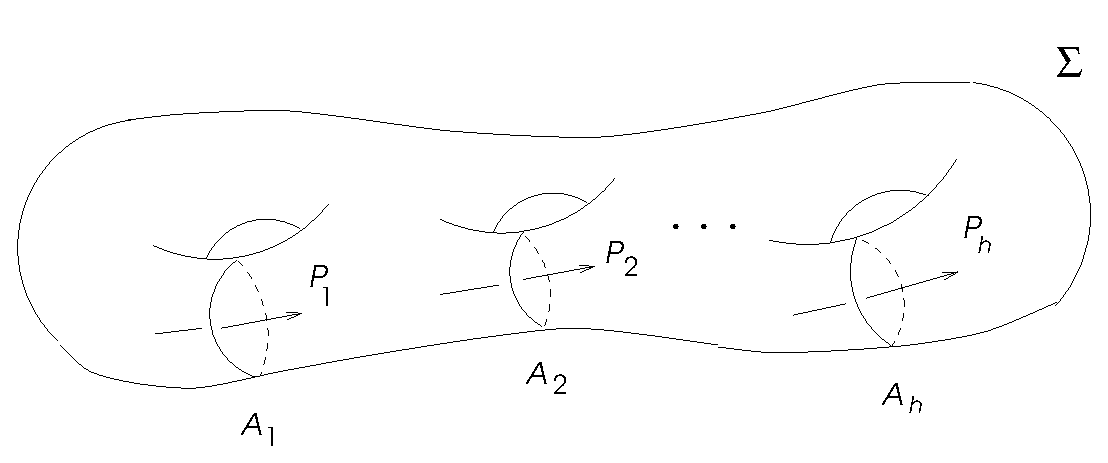
\epsfig{file=fig2.eps}}
\end{figure}

The partition function corresponding to a cylinder with boundary
conditions determined by wavefunctions $\Psi_R$ (resp. $\Psi_{R'}$) on
the two boundary components is equal to 0 if $R \ne R'$, since 
$\Psi_R$ is an eigenfunction of the Hamiltonian $H$. (See
Figure 2.)
The partition function  of a cylinder 
$S^1 \times I$ of area $\areaa$  with external states 
$\Psi_R$ on both boundary components is 
\begin{equation}
Z( S^1 \times I) = 1 \cdot 
\exp (  - \frac{e^2 \areaa \tilde{c}_2(R)} {2}  ) 
\end{equation}
(since the $\Psi_R$ are eigenstates of the Hamiltonian $H$). 
We may decompose the cylinder as in Figure 4:
this yields the partition function of the cylinder with external
states $\Psi_R$ on both  boundary components as the product of the
partition function of $\pants$ (with external states $\Psi_R $ on 
all boundary components) and that of $D$, so that
\begin{equation}
w_R \cdot v_R = 1. 
\end{equation}
To determine $v_R$, it suffices to consider a disk $D$  of very small area.
If we fix the holonomy of a connection around the boundary of $D$ to take
the value $U \in G$, the partition function for the
disk (restricting to  connections on $D$ with boundary holonomy 
$U$) is (via quantization)
\begin{equation}
Z (U) = \sum_R v_R \chi_R (U) 
\end{equation}
(where as above  $\chi_R$ denotes the character of the
representation $R$). If we instead 
 compute the partition function via the
path integral, we write the action as
\begin{equation} 
I(U) = \int_{A} \Tr (|F|^2) ,
\end{equation}
and 
\begin{equation}
Z(U) = \int DA \exp ( - \frac{1}{e^2} 
\int \Tr (|F|^2)  ), 
\end{equation}
(where we have restricted to connections for which the 
boundary holonomy is $U$). This gives 
\begin{equation}
Z(U) = \exp{\eulconst} \delta(U - 1), 
\end{equation}
(since the Euler-Lagrange equation implies that the dominant contribution
comes from flat connections, which necessarily have trivial holonomy
around the boundary of $D$). Here, $\eulconst$ is the
(as yet undetermined) constant which 
appeared in (\ref{undet}) multiplying the 
Euler characteristic of the Riemann surface.
Hence we see that 
\begin{equation}
\exp(\eulconst) \delta (U-1) = \sum_R v_R \chi_R (U). 
\end{equation}
If we multiply both sides of this equation by 
$\chi_{R'} (U)$ and integrate over $U$, using the orthogonality
relations for group characters we find
\begin{equation}
v_R = \exp (\eulconst) \dim R, 
\end{equation}
and hence
\begin{equation}
w_R = \frac{\exp ( - \eulconst)}{\dim R}. 
\end{equation}
Thus the partition function is
\begin{equation}
Z(\Sigma^g, e^2 \areaa) = 
\sum_{R} w_R^{2g-2} \exp ( - \frac{\tilde{c}_2 (R) e^2 \areaa}{2} ) 
\end{equation}
\begin{equation} 
= \sum_R \frac{ e^{-\eulconst(2g-2)}
 \exp ( - \tilde{c}_2 (R) \varepsilon/2  ) }{
(\dim R)^{2g-2} }
\end{equation}
where we have introduced $\varepsilon = e^2 \areaa$. 

\begin{figure}
\centerline{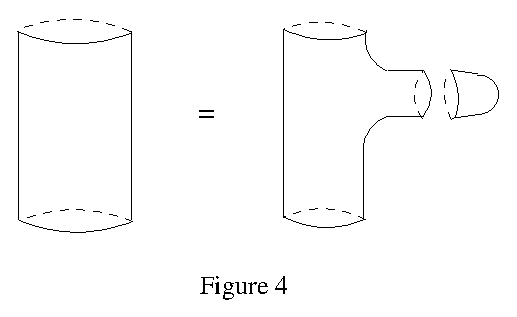
\epsfig{file=fig4.eps}}
\end{figure}

The computation we have just performed gives the sum of partition 
functions corresponding to bundles of all possible topological 
types (recall that if $G$ is not simply connected there will in general
be several topological types of bundles over $\Sigma$).
To study the contribution of one particular topological type, 
we take $G$ to be simply connected and pick an element
$\zeta \in Z(G)$.
Choosing a point $ p \in \Sigma$ we restrict to connections on 
$\Sigma - \{ p \}$ such that the holonomy around $p$ is
equal to $\zeta$. (Such a connection will descend to a flat
connection on a  quotient bundle with structure group 
$G/Z(G)$, whose topology is determined by 
$\zeta$.) In this setting we repeat the analysis above: we find that
the path integral over connections with holonomy $\zeta$ around 
$p$ is given (via quantization) by 
\begin{equation}
\sum_R u_R \chi_R (U) 
\end{equation}
and (via the path integral) by 
\begin{equation}
\exp (\eulconst) \delta (U - \zeta).
\end{equation}
 If we multiply by
$\chi_R'(U)$ and integrate over $U$ we find
\begin{equation}
u_R = \exp(\eulconst) \chi_R(\zeta) = \exp 
(\eulconst) (\dim R) \hat{\chi}_R(\zeta) 
\end{equation}
where $\hat{\chi}_R (\zeta) \in U(1)$ is the 
normalized character evaluated at $\zeta$. 
Thus the partition function becomes (since the Riemann surface
is now decomposed into $2g-1$ copies of $\cal P$ and
one copy of the disk $D$)
\begin{equation}
Z(\varepsilon, g, \zeta) = 
\sum_R w_R^{2g-1} e^{ - \tilde{c}_2(R) e^2 \areaa/2} 
u_R
\end{equation} 
\begin{equation} \labell{refg} 
 = \sum_R 
\frac{ e^{ - \eulconst (2g-2)}
 e^{ - \varepsilon \tilde{c}_2(R)/2 } }
{(\dim R)^{2g-2} } \hat{\chi_R} (\zeta). 
\end{equation}
This is the partition function for a particular class of 
$G$ bundles corresponding to flat connections
on a Riemann surface of genus 
$g$ with one boundary component and  with holonomy
$\zeta$ around this boundary component.  The
 partition function for the corresponding class of 
$G/Z(G)$ bundles on a Riemann surface of genus $g$ with 
no boundary is obtained by dividing  (\ref{refg}) by 
a factor $(\#Z(G))^{2g-2}$, since this component of the
 moduli space of flat
$G/Z(G)$ connections is an unbranched cover (of order
$(\#Z(G))^{2g-2}$)
 of the moduli space of
flat $G$ connections on a Riemann surface of genus $g$ with one
boundary component around which the holonomy is constrained to take
the central value $\zeta$.

We conclude this section by studying the example 
$G = SU(2), $ $ \zeta = - 1$. 
For each integer $n \ge 1$ there is a unique representation 
$R_n$ of dimension $n$ with $\hat{\chi_{n}} (\zeta) = 
(-1)^{n+1}$. 
The quadratic Casimir of the representation $R_n$ is 
$$c_2(R_n) = (n^2 - 1)/2; $$
this is renormalized to 
$$ \tilde{c}_2 (R_n) = n^2/2. $$
The partition function corresponding to an $SO(3)$ bundle
of $w_2 \ne 0 $ is  given (up to an overall
multiplicative normalization 
constant independent of the genus $g$ ) by 
\begin{equation}
Z(\varepsilon)  = e^{ -\eulconst{(2g-2)}} 
\sum_{n \ge 1} \frac{(-1)^{n+1} }{n^{2g-2} }
e^{ - \varepsilon n^2/4} .
\end{equation}
Let us now verify that this is 
the sum of a term which is a polynomial in $\varepsilon$ 
(the polynomial dependence being expected from 
(\ref{10.20})) and
a second term which is exponentially decaying
of order $e^{- b/\varepsilon}$ for some positive constant $b$.
We do this by differentiating the series to find  
that
\begin{equation} \labell{diffser}
\left (
e^{  \eulconst(2g-2)}  4^{g-1} 
 \frac{\partial}{\partial \varepsilon} \right )^{g-1} 
Z(\varepsilon) = F(\varepsilon),
\end{equation}
where we have defined
$$
F(\varepsilon) = \sum_{n \ge 1} (-1)^{n+1} e^{ - \varepsilon n^2/4}. 
$$
We have that
$$ 2 F(\varepsilon ) - 1 = - \sum_{n \in \ZZ} 
(-1)^n e^{- \varepsilon n^2/4}, $$
and using the Poisson summation formula this is given by 
\begin{equation} \label{poisson}
 2F(\varepsilon) = 1 - \sqrt{4\pi/\varepsilon}
  \sum_{m \in \ZZ} e^{ - (2\pi)^2(m+1/2)^2/\varepsilon}. 
\end{equation}
(The terms in the sum indexed by 
$m $   correspond to the contribution of the critical 
points of the Yang-Mills functional arising from unstable bundles
of the form $\call_m \oplus \call_{-m+1}, $ where $\call_m$ is a line bundle
over $\Sigma$ of degree $m$.)
We may now apply  (\ref{diffser}) to integrate 
(\ref{poisson}), showing that $ Z(\varepsilon)$ is the sum of a 
polynomial in $\varepsilon$ (of degree $g-1$) plus a term exponentially
decaying like $G(\varepsilon) e^{ - b/\varepsilon}$ for a positive constant $b$
(where $G(\varepsilon)$ is a polynomial 
 in $\sqrt{\varepsilon}$ and $1/\sqrt{\varepsilon}$).

\vspace{0.3in}
\noindent{\bf References:}

\noindent{\bf [AB]} M.F. Atiyah, R. Bott, The Yang-Mills equations
over Riemann surfaces, {\em Phil. Trans. Roy. Soc. Lond.} {\bf A 308}
(1983) 523-615.

\noindent{\bf [BGV]}  N. Berline, E. Getzler, M. Vergne, 
{\it Heat Kernels  and Dirac Operators}, Springer-Verlag
(Grundlehren vol. 298), 1992.

\noindent{\bf [BV]} N. Berline, M. Vergne, Z\'eros d'un
champ de vecteurs et classes caract\'eristiques
\'equivariantes, {\em Duke Math. J.}
{\bf 50} (1983) 539-549.
\smallskip

\noindent{\bf [JK1]} L. Jeffrey, F. Kirwan, Localization for nonabelian group 
actions, {\it Topology} {\bf 34} (1995) 291-327.

\noindent{\bf [JK2]} L. Jeffrey, F. Kirwan, Intersection pairings in 
moduli spaces of vector bundles of arbitrary rank over a Riemann
surface, preprint alg-geom/9608029 (1996).

\smallskip
\noindent{\bf [M] } 
A.A. Migdal, Sov. Phys. JETP {\bf 42}, 413 (1975) (Zh. Eksp. Teor.
Fiz. {\bf 69}, 810 (1975).

\smallskip
\noindent{\bf [T]} M. Thaddeus, Conformal field theory and the cohomology
of the moduli space of stable bundles, {\em J. Diff. Geom.} 
{\bf 35} (1992) 131-149.

\smallskip
\noindent{\bf [W1]} E. Witten, On quantum gauge theories in two dimensions,
{\em Commun. Math. Phys.} {\bf 141} (1991) 153-209.
\smallskip

\noindent{\bf [W2]} E. Witten, Two dimensional gauge theories revisited,
hep-th/9204083;
{\em J. Geom. Phys.} {\bf 9} (1992) 303-368.

\end{document}


